\documentclass[12pt, a4paper]{scrartcl}
\usepackage[utf8]{inputenc}
\usepackage{graphicx}
\usepackage{amsmath, amsthm, amssymb, textcomp}
\usepackage{setspace}
\usepackage{paralist}
\usepackage{graphicx}
\usepackage{caption}
\graphicspath{{WSK_im/}} %Graphic is in a folder named WSK_im in the currend directory
\usepackage{float, hyperref}
\usepackage{authblk}
\renewcommand\Authfont{\fontsize{12}{14.4}\selectfont}
\title{Bayesian probability theory - Lesson 5}

\author{Wolfgang von der Linden}
\date{Transscript}

\begin{document}
\setlength{\parindent}{0pt}
\maketitle
\onehalfspacing

Welcome to the fifth unit of the course on Bayesian probability theory. 
My name is Wolfgang von der Linden and I will enable you to help Captain Bayes and her crew to prevail on their odyssey across the ocean.
This unit is dedicated to \textbf{stochastic processes} and \textbf{random walks}. We will determine the average distance from the origin in a random walk. We will investigate the relation to diffusion. We will discuss \textbf{Markov processes} to simulate the moving pattern of the rat on the ship and we will learn how to solve probabilistic problems by computer simulations.\\

\section*{The random walk}
Let us begin this lesson with a proper description of Captain Bayes' random odyssey across the ocean as a so-called \textbf{random walk}.
We consider a regular infinite square lattice in two dimensions which represents the possible positions of the ship on the map. The spacing is 1 in arbitrary units. The ship shall start at the origin. Each possible ship position has 4 nearest neighbours that are a distance one away. Every day - which we call a step - the ship - now also called a walker -  randomly jumps to one of these nearest neighbour positions. %5_1
 \begin{figure}[H]
	\centering
	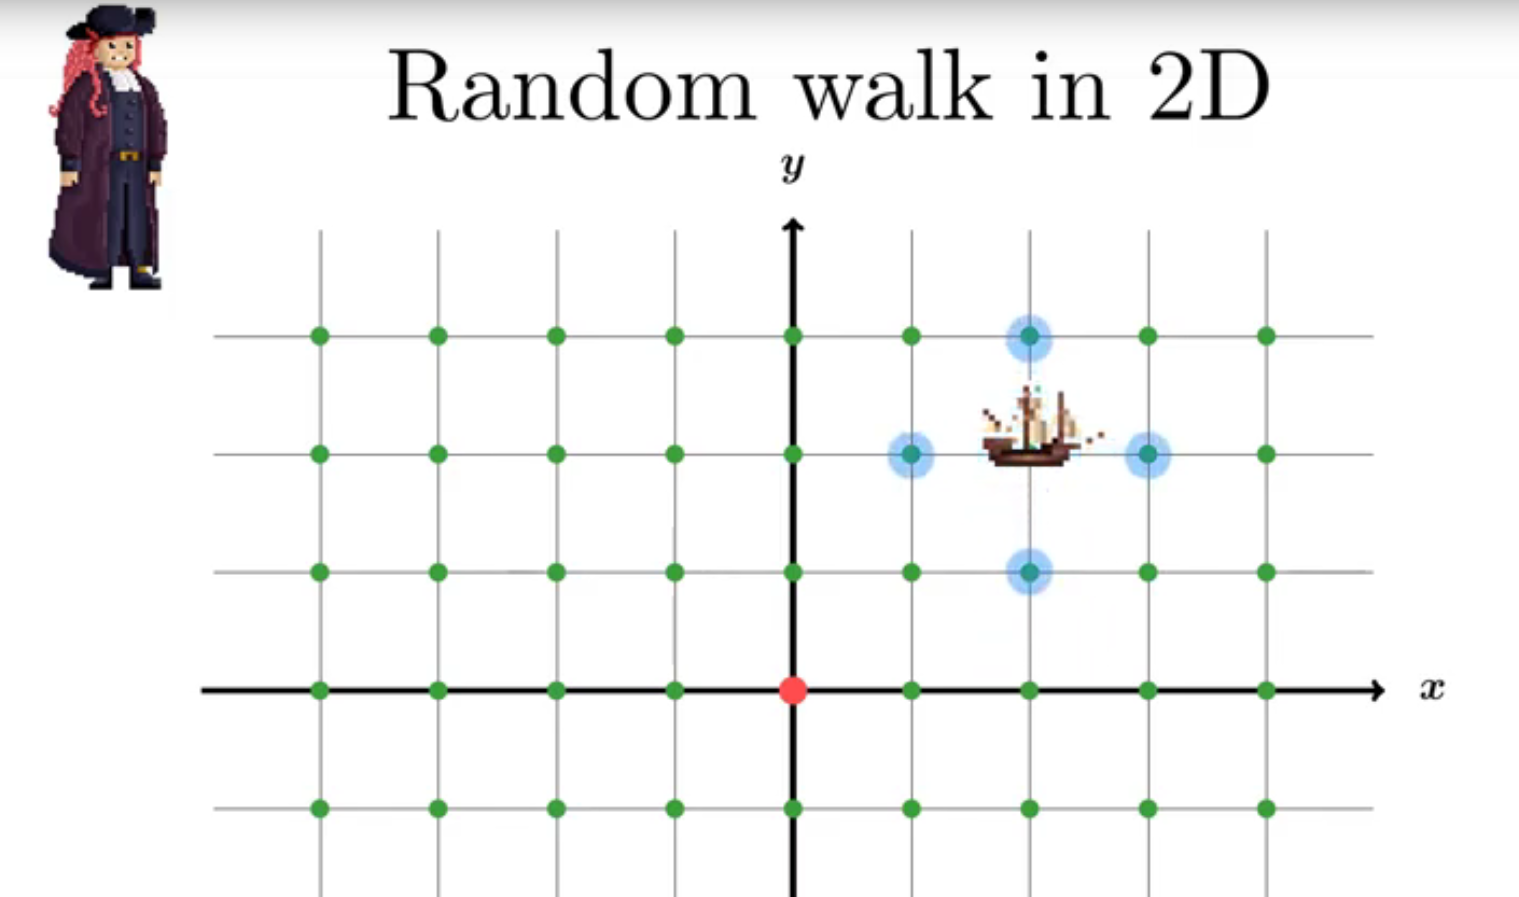
\includegraphics[width=0.75\textwidth]{5_1.png}
\end{figure}
\fbox{\parbox{\linewidth}{\textbf{Question 1.} How many possibilities are there to reachposition (2$|$1) in 3 days?\\
a) 1\\
b) 4\\
c) 3\\
d) 2
}}\\
The journey is therefore characterised by a sequence of directions the ship sails. 
We map the cardinal directions to random variables and count the frequencies $K_i$ how often a direction occurs.
There are several paths that lead to the same final position, which is given by the $x$ and $y$ coordinates that can be calculated from the \textit{frequencies of the directions}, i.e. $x = K_1-K_3$, $y=K_2-K_4$\\
 \begin{figure}[H]
	\centering
	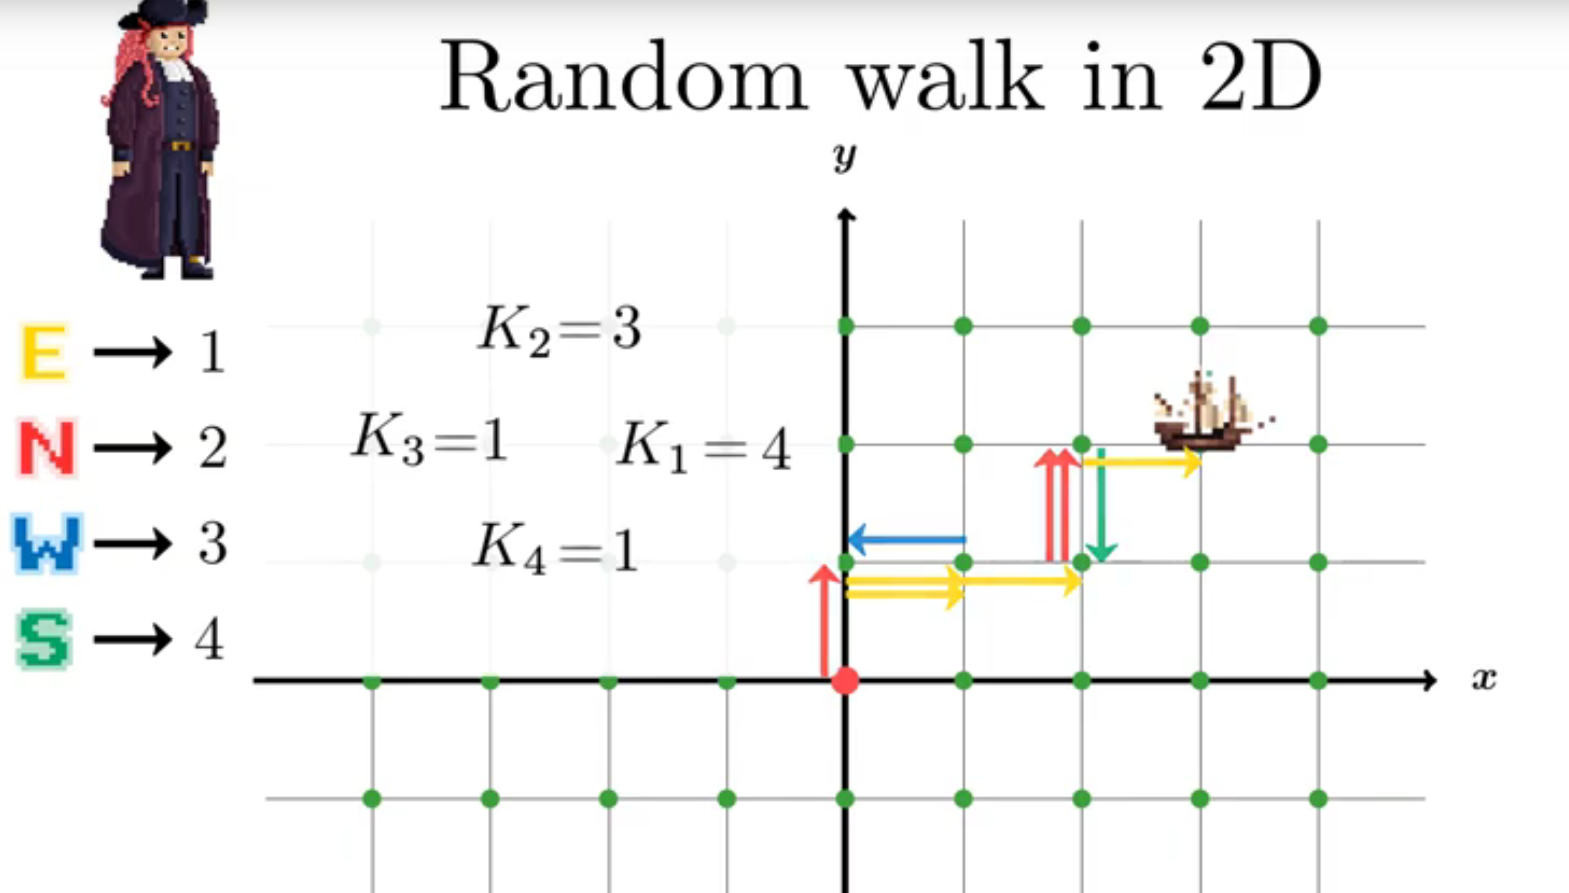
\includegraphics[width=0.75\textwidth]{5_2.png}
\end{figure}
\fbox{\parbox{\linewidth}{\textbf{Question 2.} Which of the following frequencies lead to the position (3$|$2)?\\
a) $K_1=3,K_2=0,K_3=2,K_4=0$\\
b) $K_1=1,K_2=3,K_3=2,K_4=0$\\
c) $K_1=3,K_2=8,K_3=0,K_4=6$\\
d) $K_1=5,K_2=6,K_3=2,K_4=4$\\
}}\\

The probability for such a set of direction frequencies after steps is given by the \textbf{multinomial distribution}.\\
\begin{equation*}\boxed{P(K_1,K_2,K_3,K_4|N)=\frac{N!}{\prod_iK_i!}\prod_iQ_i^{K_i}
}\end{equation*}\\
\fbox{\parbox{\linewidth}{\textbf{Question 3.} Given the following frequencies: $K_1=3,K_2=1,K_3=4,K_4=5$, what is the final position of the ship (it always starts at (0$|$0)?\\
a) (3$|$1)\\
b) (2$|$-1)\\
c) (-1$|$-4)\\
}}\\
\fbox{\parbox{\linewidth}{\textbf{Question 4.} Given the same frequencies: $K_1=3,K_2=1,K_3=4,K_4=5$, how many different paths can be realized with those frequencies?\\
a) 360360\\
b) 210\\
c) 3422\\
}}\\

The compass is perfectly symmetric so by the \textbf{principle of indifference} all four directions have the same probability of $P=0.25$\\
\textit{Note: You can become creative and change the probabilities of the compass - maybe making them also dependent on the position of the ship - to study for instance the effect of an ocean shift or ocean streams}.\\
%%%%%%




What we have derived just now is a so-called \textbf{random walk} which is a special case of a \textbf{stochastic} or \textbf{random process}. Such processes are in most cases \textit{time or space dependent random variables}. In our case it is the time-dependent sequence of random positions of the ship on the map. If it depends on space, it is also called a \textbf{random field} in modern literature.
Stochastic processes are widely used to model and analyse complicated systems such as stock market prices, the motion of particles in a liquid or the spacial random variation of geological material to study the origin of earth quakes.
The properties of stochastic processes can be studied numerically by using many repeated realisations of one walk or by using many walkers in parallel.
Furthermore, stochastic processes are also used to solve high dimensional problems that originally have nothing to do with chance.  Like the evaluation of high-dimensional integrals or the solution of partial differential equations.\\

\section*{The final position}
We will now discuss the general statements we can make about Captain Bayes' random odyssey.\\
\textit{Which final position do we expect on average after N days steps if many ships walkers would start at the same time and same initial position?}
The \textbf{mean value} in x-direction is given by the \textit{mean of the difference of the direction frequencies} \[\langle K_1\rangle-\langle K_3\rangle\]. By using linearity we can conclude that the mean position is 0. 
\textit{That does not mean that on average a single walker does not move!}
It rather means that if you repeat the random walks many times, the mean of the final positions will be zero. 
Here is an extreme example in 2 dimensions: one ship walker may end at (N,0) and another one at (-N,0). Their mean value is zero, although they have traveled individually to the furthest possible points.\\
Bernoulli wanted to know the \textit{average distance they reach from their origin after N days}. Obviously, the mean position is not the right object to answer this question. Instead we’d rather use the \textbf{mean of the quadratic distance} \[\langle x^2\rangle = \langle K_1^2\rangle + \langle K_3^2\rangle-2\langle K_1K_3\rangle\] and take the square root, since this provides a suitable distance measure.
We can split K into the mean plus a fluctuation $K_i=\langle K_i\rangle +\Delta K_i$
So (after a somewhat lengthy calculation) the mean squared distance is equal to the number of steps $N$.
Therefore, the answer to Bernoulli's question is: 
\textit{The mean distance is given by the square root of the number of steps.}\\


As usual, Captain Bayes wanted to delve deeper and asked about the \textit{probability for the position}. The answer is particularly transparent in 1 dimensions where we use a compass that has only the two directions West and East.
Then we can express the x-position after N steps by the difference of the number of steps $K_i$ taken in these directions.
To reach position x in N steps, the number of times the compass points to the west must be $K_{West}$.
\begin{equation*}\boxed{x = K_{East} - K_{West} = N - 2K_{West}\Rightarrow K_{West}=\frac{N-x}{2}
}\end{equation*}\\
As the frequency to dial K times "West" on the random compass is given by the \textbf{binomial distribution}, the same holds true for the position.
\begin{equation*}\boxed{P(x|N)={N\choose \frac{N-x}{2}} 2^{-N}
}\end{equation*}\\
Note that in an even or odd number of steps, only an even or odd site can be reached.
For the 2D case we will use \textbf{Markov processes} and matrices to determine the probability for the position.\\

\section*{Diffusion as a random walk}
Captain Bayes also speculated that \textit{diffusion is a random walk} too. That is indeed the case.
Diffusion is actually a motion in continuous space and time, but we will introduce finite time steps $dt$. Within such a time step two things can happen. Either the particle \textit{hops a distance $dx$} in one of the Cartesian directions or it \textit{stays where it is}. We make the obvious assumption that the hopping probability is proportional to the time interval $dt$.
Then, the probability that \textbf{no hopping} occurs in dt is (1 - P(hopping)). %5_3
 \begin{figure}[H]
	\centering
	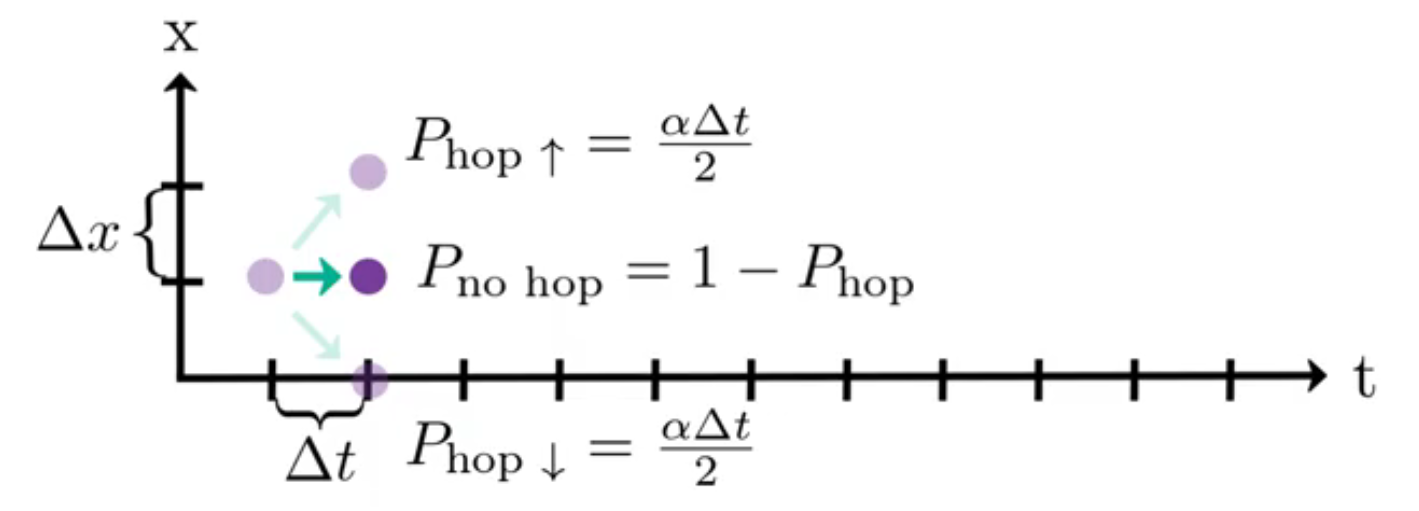
\includegraphics[width=0.75\textwidth]{5_3.png}
\end{figure}
That defines the random walk. The only difference to the previous case is the possibility that the walker does \text{not} move in each time step, which would correspond to the free day Bernoulli is longing for.
The trick now is to express the probability to reach position $x$ at time $t$ via the \textit{marginalization rule} as a sum over probabilities for the position $x’$ at time $t-dt$ times the hopping probability from $x’$ to $x$ in one time step $dt$. That leads to a recursion relation. 
\begin{equation*}\boxed{P(x,t)=\sum_{x'}P(x,t|x',t-dt)P(x',t-dt)=(1-\alpha\Delta t)P(x,t-dt)+\sum_{|x-x'|=\Delta x}\frac{\alpha\Delta t}{2D}P(x',t-dt)
}\end{equation*}\\
The same trick will be discussed in greater detail in case of the Markov process. Here we are more interested in the final result.
Rewriting the recursion relation and taking the appropriate limit $dt\rightarrow 0$ and $dx \rightarrow 0$ leads to the (to physicists) well known diffusion equation.
\begin{equation*}\boxed{\frac{\partial}{\partial t}\rho(x,t)=\alpha \frac{\partial^2}{\partial x^2}\rho(x,t)
}\end{equation*}\\
Here, $\alpha$ is the \textit{diffusion constant} and $\rho$ stands for the \textit{probability to find the particle at time t at position x}. But as we discussed in the second unit it can also be interpreted as relative frequency. So if there is a huge number of particles in the system described by their density, the diffusion equation is equally valid for the density.
Let us think of a drop of ink that is put on the water surface. Initially the size is almost zero. 
For this initial value problem the solution of the diffusion equation on the water surface is a 2 dimensional Gaussian.
It is centred at the origin and the variance grows proportional to time.%5_4
 \begin{figure}[H]
	\centering
	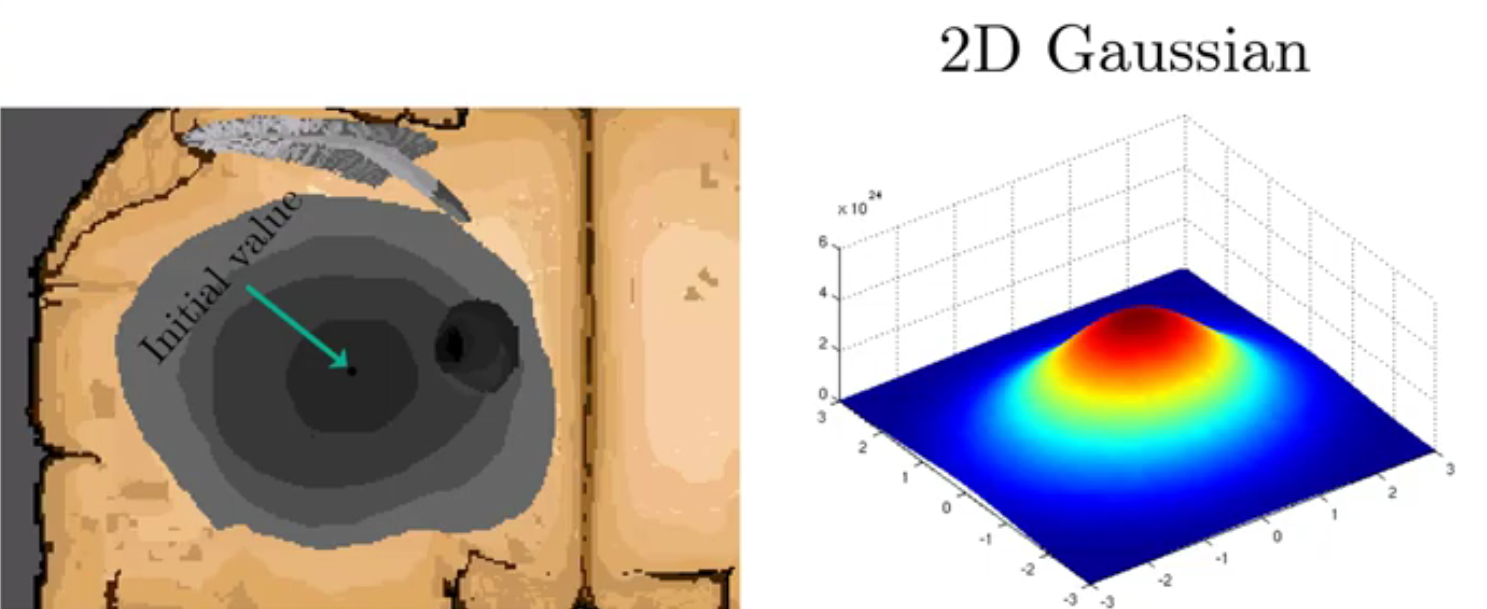
\includegraphics[width=0.75\textwidth]{5_4.png}
\end{figure}
So Captain Bayes correctly concluded that diffusion can be described by a random walk.\\


\section*{Returning to the starting point}
Pascal raised the question, whether they will ever see the bottle that she put in the ocean again.
Assuming the ship is on a daily random course the question concerns the\textit{ probability that a random walk will return to its starting point}. 
To answer this question we consider the probability that an isotropic random walk will return to its starting point after a certain number of steps.
We introduce the following proposition $a_N$ and its probability $P(a_N)$ of having an arbitrary return after N steps, which includes the possibility of having already seen the bottle in less than N steps as well.
The return always requires an \textit{even number of steps}, N=2M, so we introduce the variable M, because the return implies that for each Cartesian axis the walker moves forward as often as backward.
In 1D the frequency going East is simply half the number of total steps and the probability is given by the \textbf{Binomial distribution}.
But how does one answer the question whether the walker will ever return home? One could come up with the idea of \textit{summing over M from 1 to infinity}, since this covers all possibilities for a return - after an even number of steps. %5_5
 \begin{figure}[H]
	\centering
	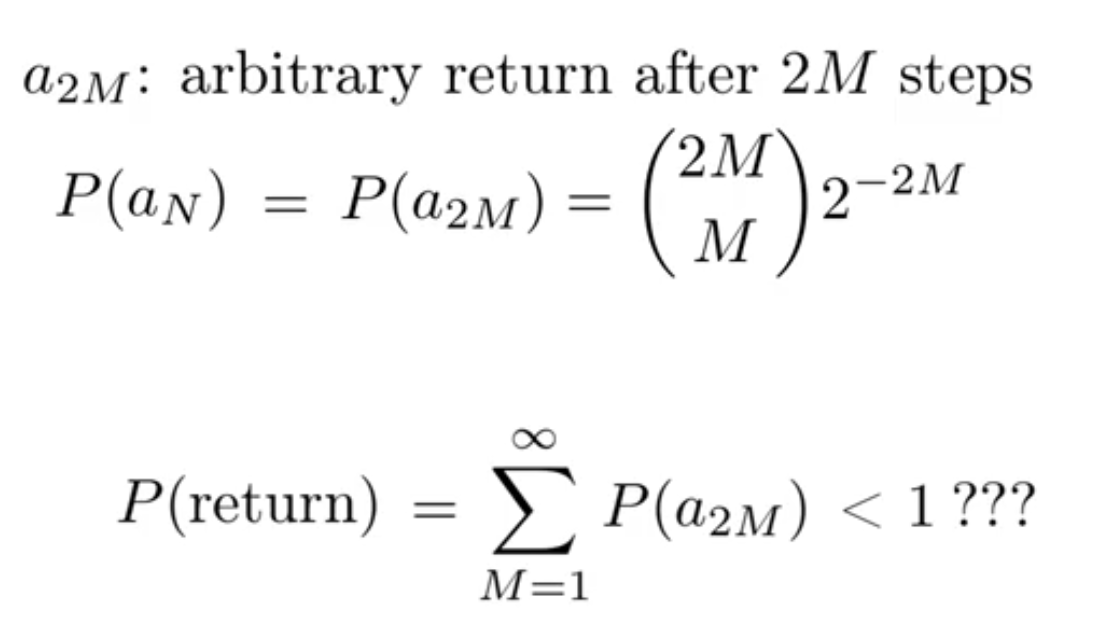
\includegraphics[width=0.75\textwidth]{5_5.png}
\end{figure}
If the sum is less than one, then the probability that the walker will never return is not-zero.
But, unfortunately, the events of arbitrary return are not exclusive since we may \textit{double count paths that} reach the origin and the sum over M does not have the desired meaning.\\

What we need instead is the probability for the \textbf{first return after N steps}.
There is a clever way to compute it. The first part of an arbitrary return is always a first return $f_K$. If the arbitrary return occurs after N = 2M steps, the first return may happen at K steps, and the remaining steps again describe an arbitrary return.
So we can \textit{decompose} any arbitrary return into first return and remaining arbitrary returns.%
\begin{equation*}\boxed{a_{2M}=\bigvee_{L=1}^{M}(f_{2L}\wedge a_{2(M-L)})
}\end{equation*}\\
This equation can be solved for the desired probability of first return by what is called the \textbf{generating functions} or a \textbf{Fourier transform}. After a somewhat lengthy calculation summing all probabilities of first return, it yields the probability to ever return - which in \textbf{1D and 2D} is equal to 1.%5_6
 \begin{figure}[H]
	\centering
	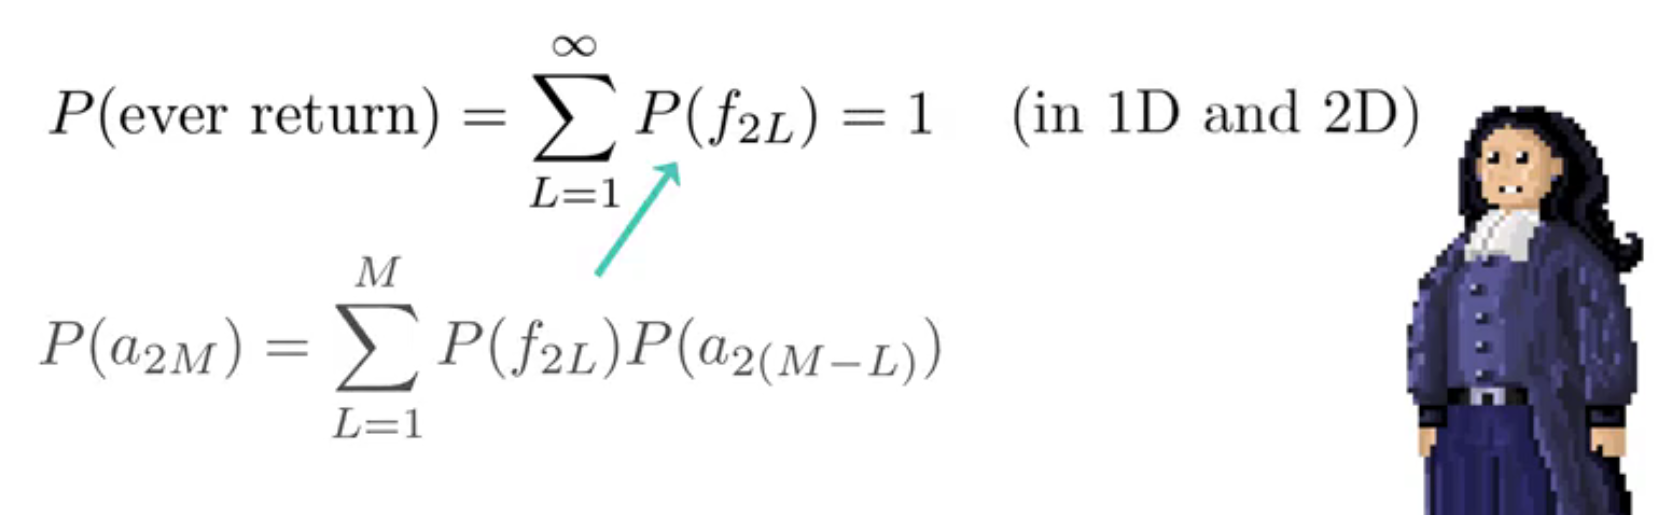
\includegraphics[width=0.75\textwidth]{5_6.png}
\end{figure}
Pascal will definitely see her bottle again, but it may take a very long time.
But what about Ernesto, will he ever return home if he follows a \textbf{3D random walk}, which may happen if he ate too many overripe grapes?
In that case the probability to ever return is less than one (34\% to be precise).
Poor Ernesto, if he is drunk the chances are 66\% that he will get lost.
\textit{So never get drunk in three dimensions}!\\


\section*{Reaching turtle island}
Bernoulli wanted to know the \textit{chance to reach turtle island that is 5 steps away within 5, 6, up to 10 days}.
Similarly to the ideas of the First return we can at least say the following immediately: It takes an odd number of days as the distance is odd - just think of a checkerboard with the colors corresponding to the even or odd days.%5_7
 \begin{figure}[H]
	\centering
	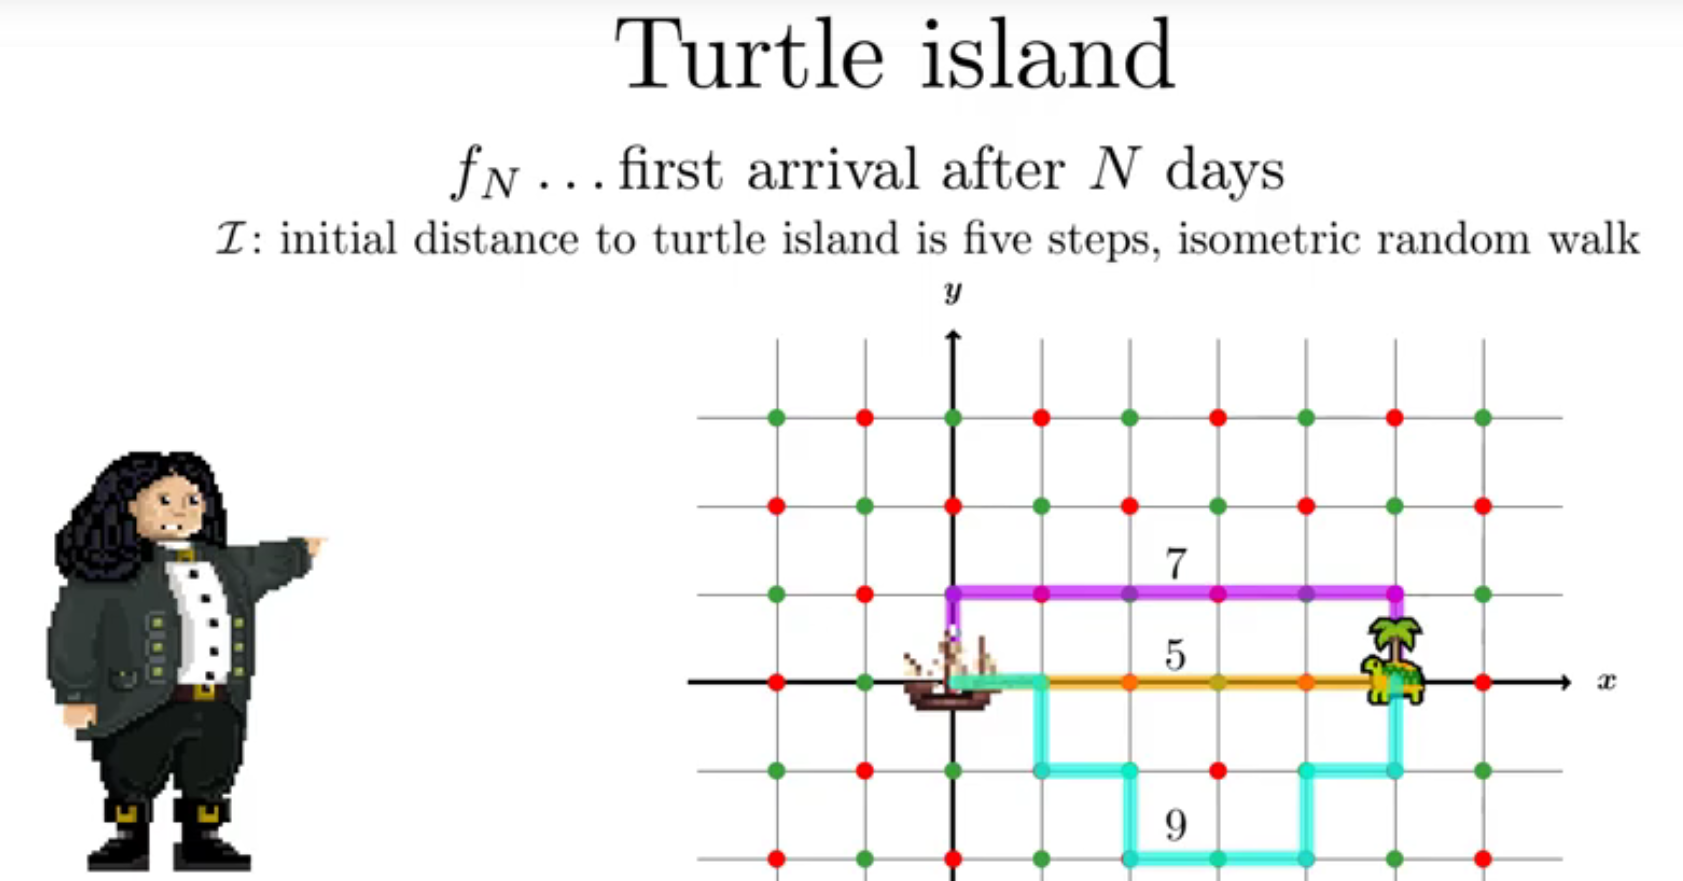
\includegraphics[width=0.75\textwidth]{5_7.png}
\end{figure}
To reach the island in 5 days if it is 5 steps away means that the ship has to go straight. 
So there is only one favourable path out of $4^5$. Thus the probability is
$4^{-5} = 0.001$ which is surprisingly small.
For the other cases one has to examine \textit{all combinations of direction frequencies $K_i$ that lead to the final position after N steps}.
As mentioned before the probability for such a combination is given by the \textbf{multinomial distribution}. Although the tricky thing is again that we are considering paths with arbitrary arrivals and not those with first arrival, but Bernoulli will definitely disembark as soon as he reaches the island. 
So we have to subtract those paths which already have reached turtle island or use the same convolution trick we saw before.
\begin{equation*}\boxed{P(f_N)=\left(\frac{N!}{\prod_i K_i!}-\#\text{paths through turtle island}\right)\prod_i Q_i^{K_i}
}\end{equation*}\\
Besides the analytical version there are also other ways to solve this problem, one by using a \textit{computer simulation} using many walkers to count the relative frequencies of arrival, and one based on \textit{Markov matrices} and working with probability distributions which we will discuss just now.\\ \textit{Have a look at the Pluto notebooks that show you these different solutions and other simulation techniques!}\\

\section*{Markov processes}
There are many different important types of stochastic processes. Those discussed so far have one thing in common: The state or position of the next time step depends only on the previous position, so there is \textit{no memory}. A journey with memory could be that Captain Bayes choses the next direction with a probability that she favours directions that occurred less frequently in the last 10 days.
A stochastic process whose \textit{next state only depends on the present state} is called \textbf{Markov process}. 
We can exploit the Markovian property to derive a recurrence relation, as we did for the diffusion problem. 
Let $x_t$ be the proposition describing for instance the position of a particle at time $t$. Time shall be discretised in units of $dt=1$. The probability for the position at time $t+1$  can then be related to the probability for the position at time $t$ via the marginalization rule.
In the case of the random walk the \textit{sum is restricted} to positions that are nearest neighbours of the final position.
\begin{equation*}\boxed{P(x^{(t+1)})=\sum_iP(x^{t+1)}|x_i^{(t)})P(x_i^{(t)})=\sum_{|x^{(t+1)}-x_i^{(t)}|=\Delta x}P(x^{t+1)}|x_i^{(t)})P(x_i^{(t)})=
}\end{equation*}\\
Since in the present example the hopping probabilities are not time dependent, we have a so-called \textbf{homogeneous} Markov process.  An example for an \textbf{inhomogeneous} Markov process would be given if there is a storm or an ocean current that influences the hopping probabilities.\\

\fbox{\parbox{\linewidth}{\textbf{Question 5.} Which realizations of an ocean current or defect on the ship are still Markovian?\\
a) The rudder for steering the ship is damaged, so the probability for turning left is always smaller than for turning right.\\
b) When hitting the coral reef on position (-2$|$2), the rudder gets damaged and the ship loses its ability to tack against the wind coming from north, so the probability for north decreases whereas all other directions become more likely.\\
c) After 10 days a storm came up, changing the probabilities for going north (decreased) and south (increased).\\
d) The probability for sailing west increases and east decreases as soon as the ship enters a y coordinate larger than 3.
}}\\

\section*{The rat problem}
The possible positions of the rat can be enumerated by an index $i$. %5_8
 \begin{figure}[H]
	\centering
	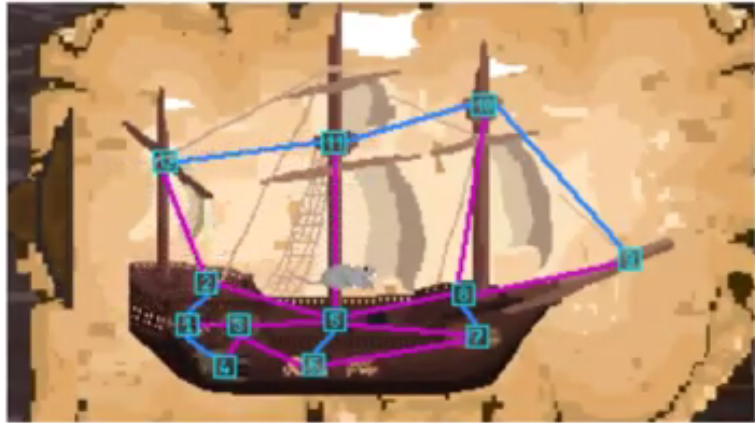
\includegraphics[width=0.75\textwidth]{5_8.png}
\end{figure}
Then the recursion relation can be expressed by matrix-vector multiplications. 
\begin{equation*}\boxed{\vec{P}^{(t+1)}=M\vec{P}^{(t)} \qquad \text{where} P_i^{(t)}=P(x^{(t)}=x_i)
}\end{equation*}\\
Here M is the so-called \textbf{Markov matrix}.
\begin{equation*}\boxed{ M_{ij}=P(x^{(t+1)}=x_i|x^{(t)}=x_j)
}\end{equation*}\\

As an example, let us consider the rat as a creature without memory that decides the next move randomly \textit{based only on the current position and nearby positions that are in range}. Each such move may have its \textit{individual probability}, perhaps depending on the odor gradient. \\
%5_9
 \begin{figure}[H]
	\centering
	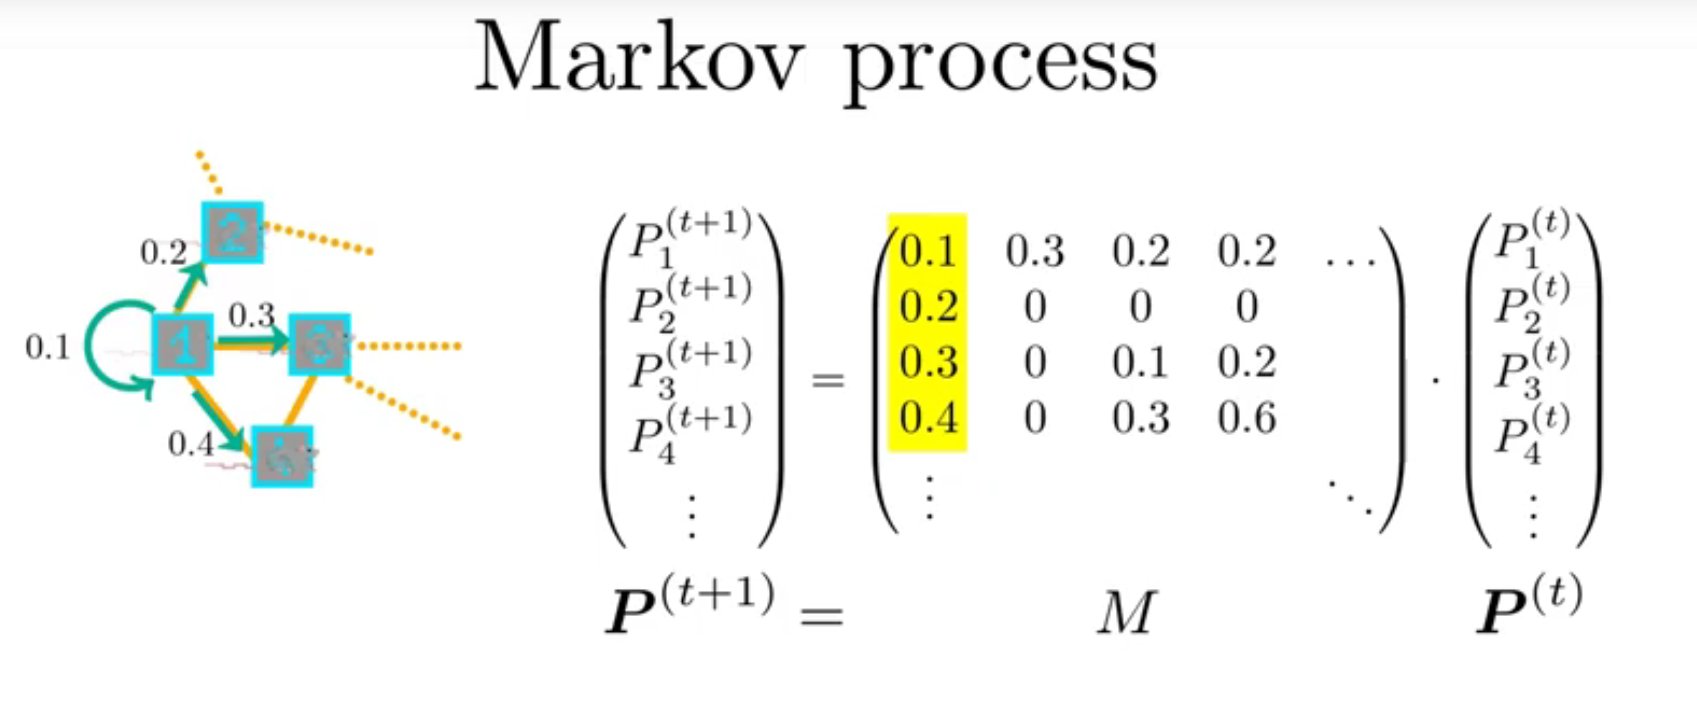
\includegraphics[width=0.75\textwidth]{5_9.png}
\end{figure}

We cannot avoid introducing at least one more definition: \textbf{Ergodicity}.\\
A Markov process is \textbf{ergodic} if there is a \textit{nonzero probability} for reaching every state $\xi_{j}$ from every other state $\xi_{i}$ in a \textit{finite} number of steps. \\%box
In the case of the rat, there could be certain disjoint areas on the ship between which the rat cannot switch.
The key object we want to determine with Markov processes is the \textit{probability distribution of the position of the rat after t time steps when we know its starting point}.\\
At time $t=0$ the probability vector has one non-zero entry only at the position of the origin. At any later time t the probability vector follows from the recursion relation.%5_10
 \begin{figure}[H]
	\centering
	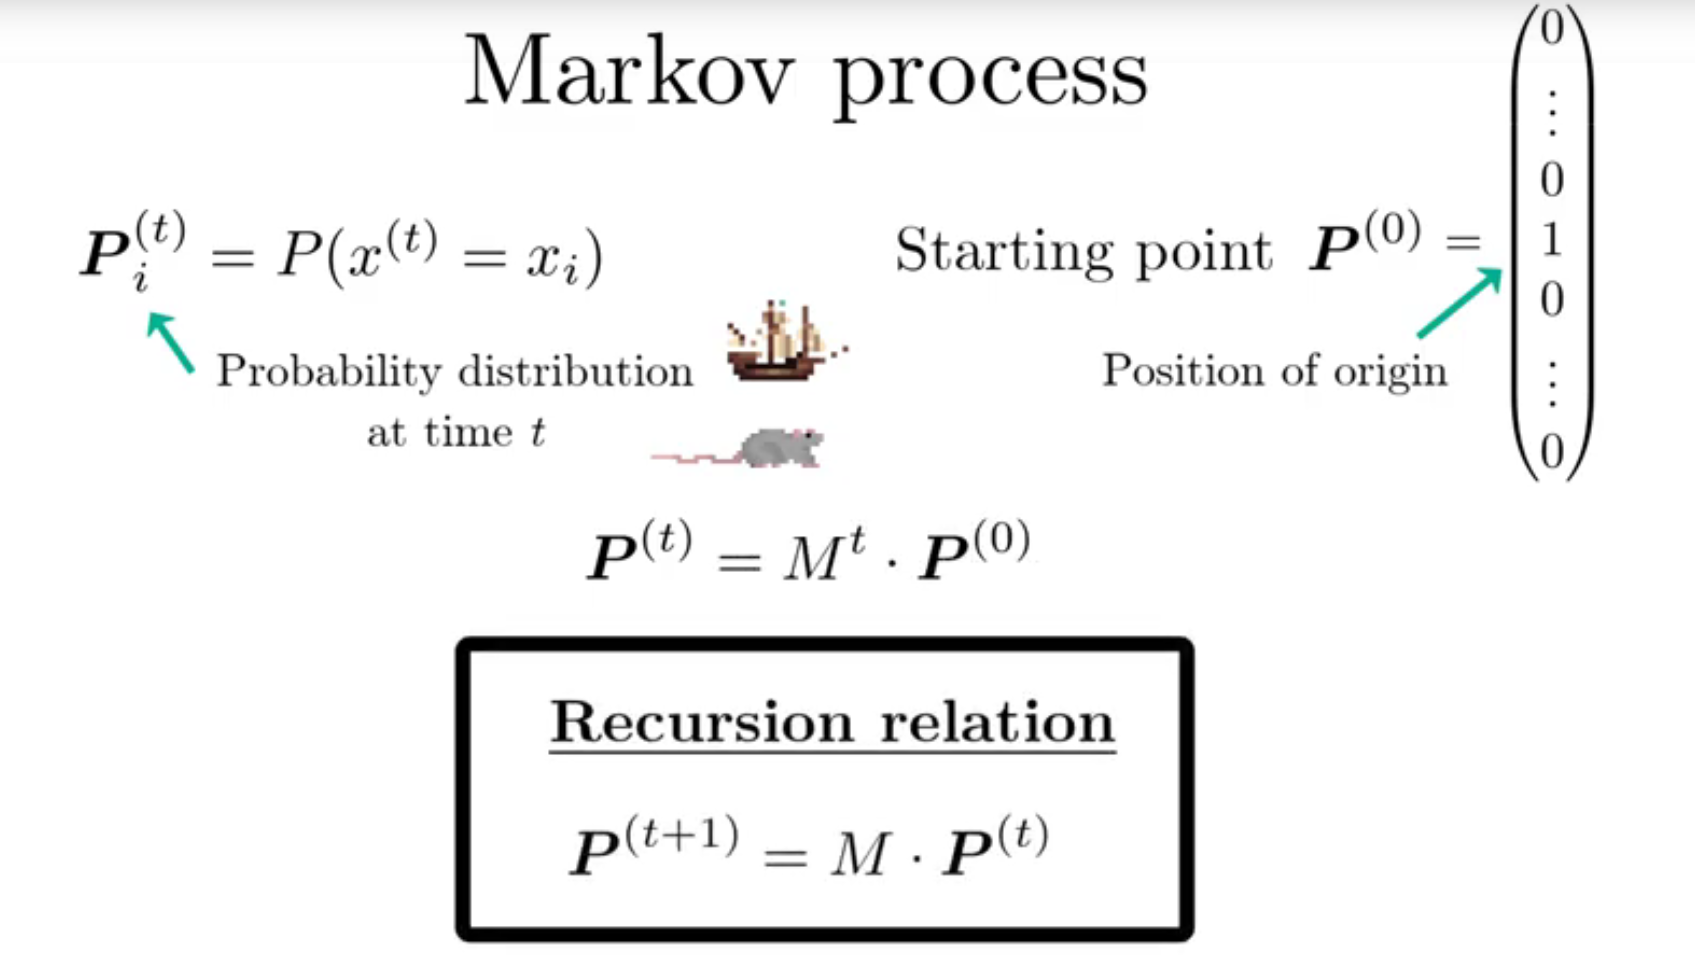
\includegraphics[width=0.75\textwidth]{5_10.png}
\end{figure}
So this illustrates how Markov processes can be used. You can also treat the question of first return or first arrival by the Markov matrices or one can generalise the concept to more general hopping probabilities.\\
\textit{In the interactive notebooks you can examine how to derive these Markov matrices and how to apply them.}\\

 \section*{Poisson processes}
Another stochastic process is the \textbf{Poisson process}, which in contrast to the random walk does not choose a random direction but a \textit{random length of the next step} at which an event happens or a \textit{random number of events that happen at the next time step of equal length}.%

Figuratively speaking, it’s a special staircase, where each step height is one but the step length is a random variable with an exponential distribution. Alternatively, one could always use the same step length but the step height is taken from a poisson distribution. With each realisation we obtain a new staircase.%5_11
 \begin{figure}[H]
	\centering
	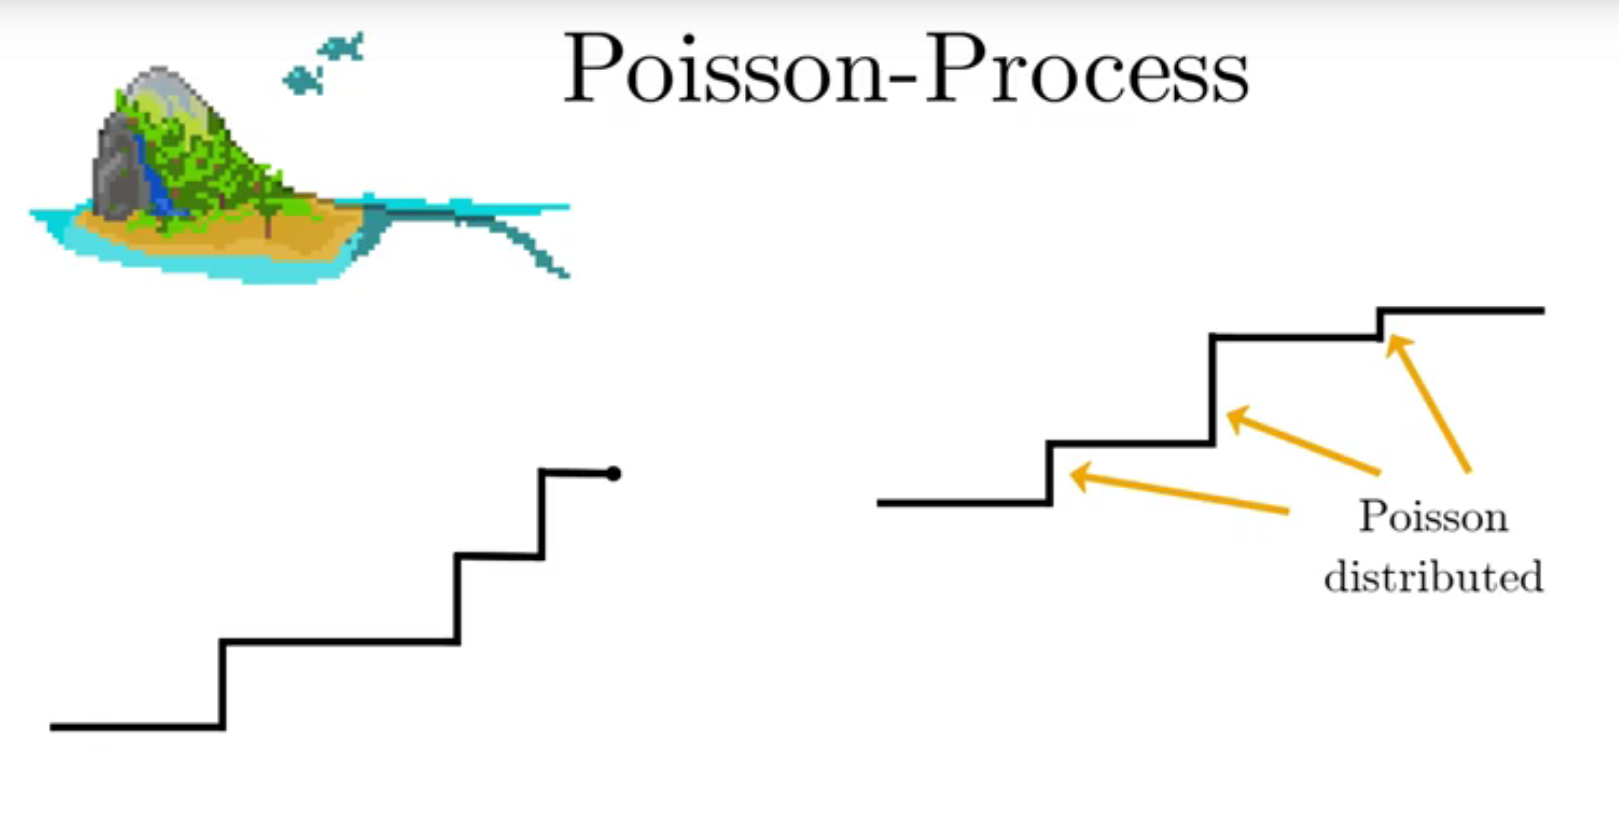
\includegraphics[width=0.75\textwidth]{5_11.png}
\end{figure}
Poisson processes play an important role in \textit{queuing theory} or in \textit{insurance} to describe the distribution of special events such as accidents.\\

\section*{Gaussian processes}
Now we turn to \textbf{Gaussian processes}. They are a special type of stochastic processes that are very \textit{versatile} and also allow for non-Markovian properties where one can \textit{choose parameters that describe the correlation} of the random variables.
For easier understanding we will give a \textit{specialised and simplified definition} of a Gaussian process that nevertheless covers most applications.
The index of the random variable $X_t$ shall be time and we only consider a finite set of discrete times (not necessarily equi-distant), the generalization to space or other index sets is obvious.
The vector formed by the corresponding random variables is \textbf{multivariate Gaussian}.
A multivariate Gaussian is given by %5_12
 \begin{figure}[H]
	\centering
	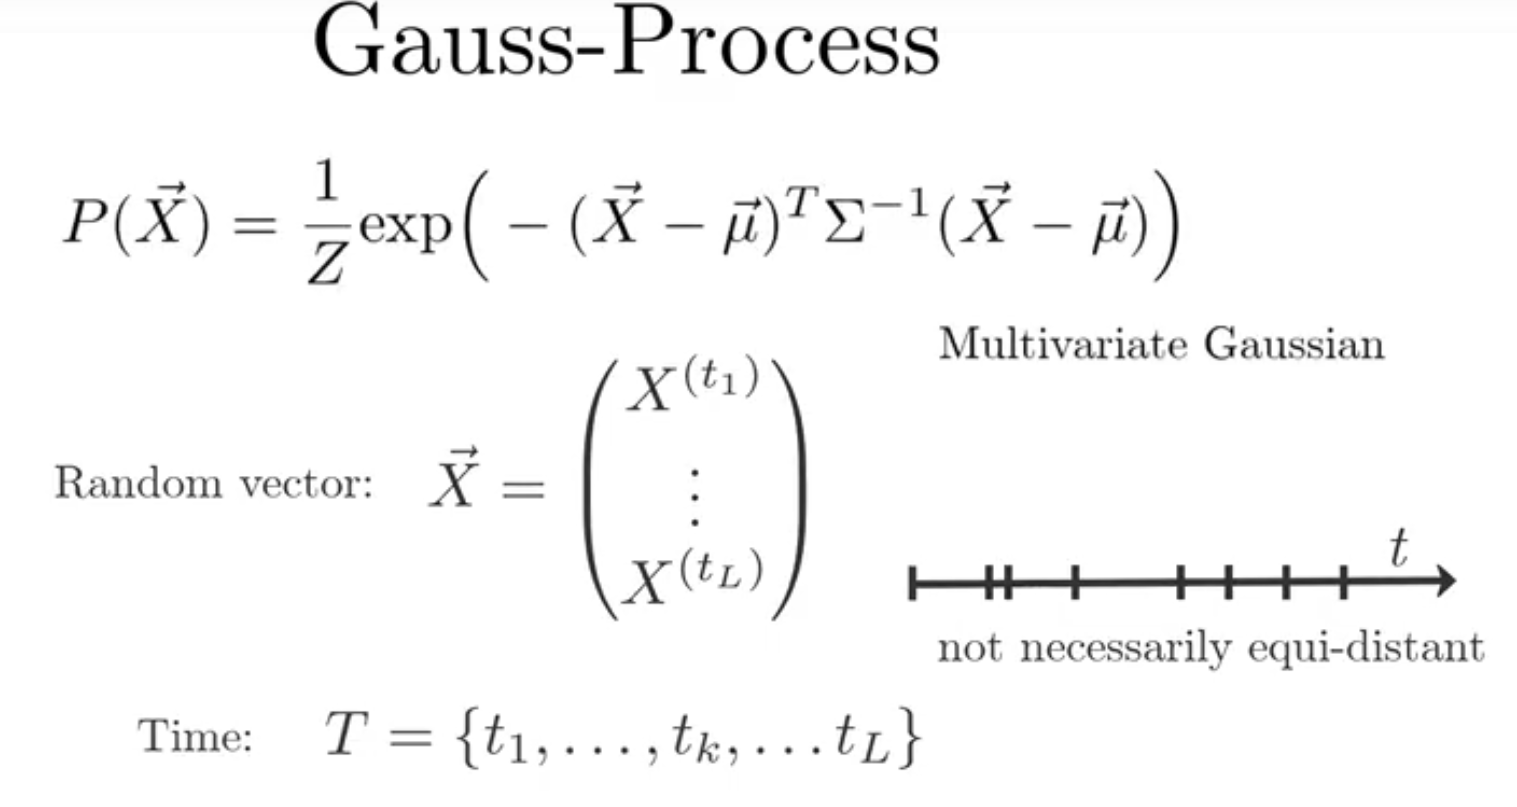
\includegraphics[width=0.75\textwidth]{5_12.png}
\end{figure}
 and it is characterized by its \textit{mean $\vec{\mu}$ and its covariance $\Sigma^{-1}$},
For the case of a one-dimensional random walk the elements of the vector are the positions at the discrete times.  
The power of Gaussian processes is due to the \textit{wide variety of forms} that can be achieved by different choices of the covariance or kernel function defining the elements of covariance matrix.%5_13
 \begin{figure}[H]
	\centering
	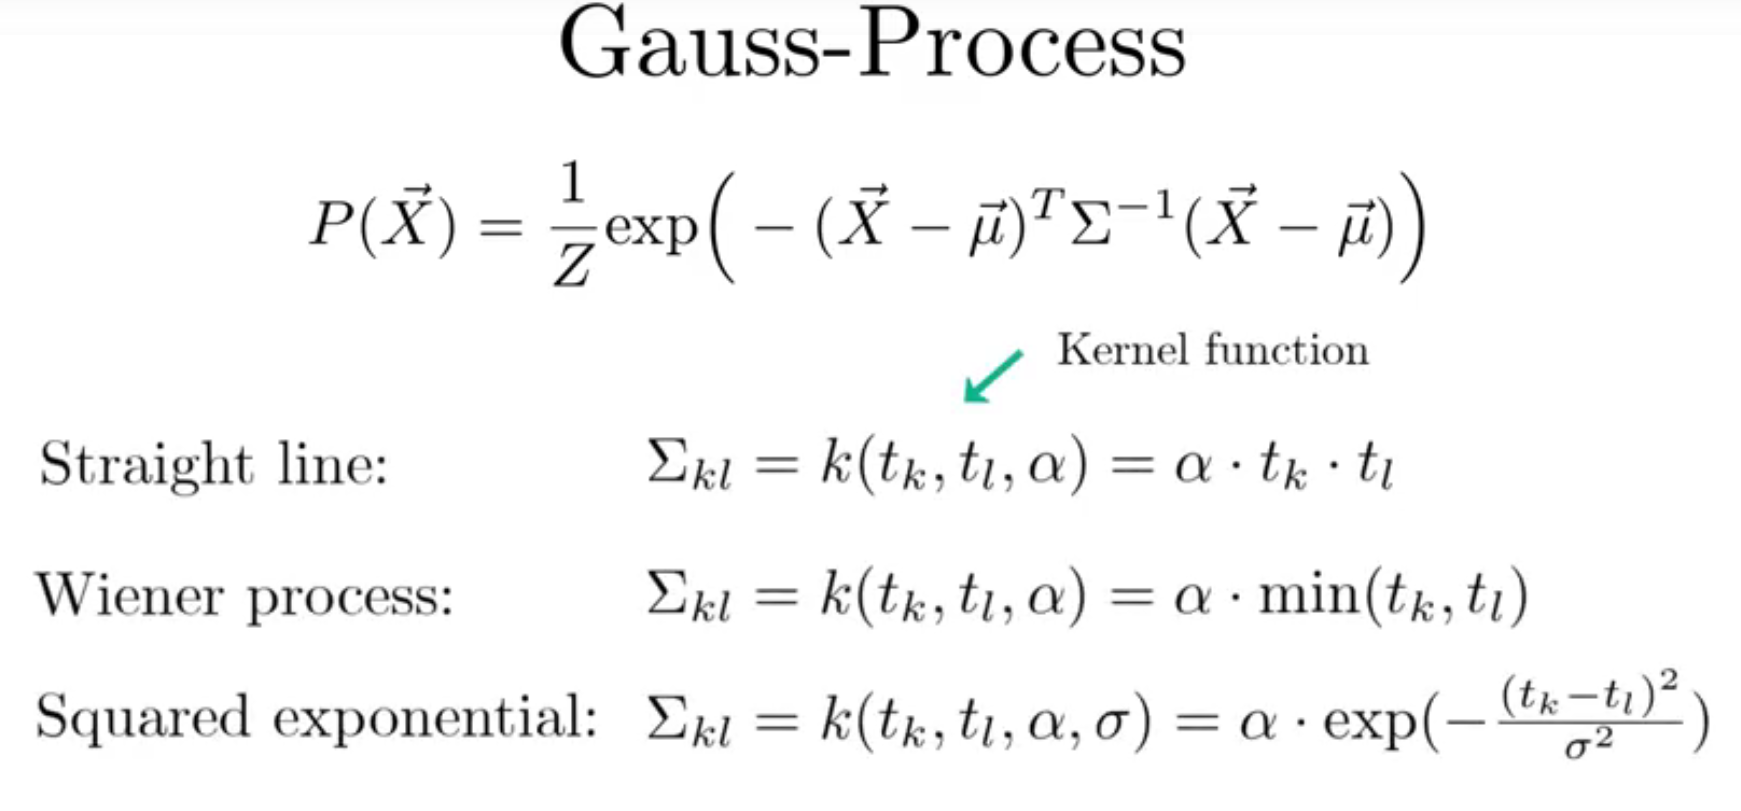
\includegraphics[width=0.75\textwidth]{5_13.png}
\end{figure}
I guess it will surprise you to hear that straight lines can be the result of a Gaussian process as well as the random walk, just due to the proper choice of the kernel function.\\
\textit{In the Pluto notebook you have ample opportunity to get acquainted with various kernels and types of results you can describe by them}.\\


\section*{Epidemics as a random walk}
Yes indeed, the spread of an epidemic can also be simulated as a random walk.
Initially there is one person that has the virus.
On each site the walker reaches, there is either a person or not, depending on the population density and it can either be susceptible for the virus, or immune. If this person also gets infected there is a second contagious walker. After 7 steps / days an infected walker becomes immune.
The epidemic spread can also be treated by probabilistic means in terms of the so-called \textbf{SIR equation} that describes the time-evolution of the probabilities for Susceptible, Infected, and Recovered (immune) people.  \\
As it would be beyond the scope of this imoox course to discuss the derivation and solution of the SIR equation in more detail, we refer to a nice youtube video for more details:
\url{https://www.youtube.com/watch?v=gxAaO2rsdIs (3b1b)}\\


This brings us to the end of Lesson 5.
We have gained some insights into how to use stochastic processes to model real life applications. Now it's your turn to deepen your understanding of these processes by going through the interactive notebooks, revisiting some of the derivations, and reviewing the additional resources. 
Please feel free to ask questions in the forum and feel encouraged to test your knowledge in the quiz!
 \begin{figure}[H]
	\centering
	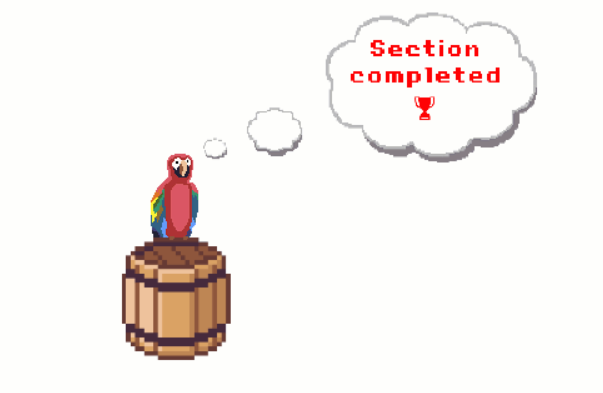
\includegraphics[width=0.75\textwidth]{5_14.png}
\end{figure}



\end{document}